% ======================================================================
%  5. Separation of concerns: prior-guided optimization
% ======================================================================
\section{Separation of concerns: prior-guided optimization}
\label{sec:contrib-prior}

The third instance concerns prior knowledge. In the laboratory, previous
experiments often suggest that effective stimulation parameters lie in a
particular region. The separation-of-concerns question becomes: should this
knowledge modify the \emph{model} of the biological response, or only guide the
experimental \emph{policy}?

\subsection{Two meanings of ``prior'': spatial vs functional}
\label{sec:contrib-prior-two}

The distinction drawn in Section~\ref{sec:bg-prior} is the crux. A
\emph{spatial} prior $\pi:\X\to[0,1]$ says \emph{where} the optimizer is likely
to lie; a \emph{functional} prior says something about the \emph{shape} of $f$
over the whole domain. They encode different information:
\begin{center}
\emph{Knowing that $x^\star$ probably lies in a region does not determine the
amplitude, smoothness or global geometry of $f$.}
\end{center}
This motivates the principle: prior information about the desired solution should
influence the decision rule when possible, without unnecessarily modifying the
statistical model of $f$. We again compare a \RIGHT{} strategy (prior in the
acquisition, generic GP on $f$) with a \WRONG{} strategy (prior injected into the
GP mean). \hfill\Psynth

\subsection{\RIGHT: the prior in the acquisition ($\alpha$-$\pi$BO)}
\label{sec:contrib-prior-right}

The spatial weight of Guay Hottin et al.~\cite{guayhottin2025},
$w_\alpha(x)=(1-\alpha)+\alpha\pi(x)$, satisfies $1-\alpha\le w_\alpha(x)\le1$,
so it can bias but never eliminate any region. We use it as prior work
(Section~\ref{sec:bg-prior}). \hfill\Plit

Multiplying the \emph{entire} UCB by $w_\alpha$ also multiplies the posterior
mean, which breaks the clean optimism argument. To obtain a transparent
guarantee we let the prior modulate only the exploration bonus, giving an
$\alpha$-\textsc{prior}-UCB rule
\begin{equation}
  a_t^{\RIGHT}(x) \;=\; \mu_{t-1}(x)+\frac{w_\alpha(x)}{1-\alpha}\,
                       \sqrt{\beta_t}\,\sigma_{t-1}(x),
  \qquad 1\le\frac{w_\alpha(x)}{1-\alpha}\le\frac{1}{1-\alpha}.
  \label{eq:prior-right}
\end{equation}

\begin{proposition}[Safe UCB adaptation, {proof in Appendix~\ref{app:prior}}]
\label{prop:prior-safe}
Under the standard confidence event, the rule~\eqref{eq:prior-right} yields
instantaneous regret $r_t\le\frac{2-\alpha}{1-\alpha}\sqrt{\beta_t}\sigma_{t-1}(x_t)$
and hence $R_T=\widetilde O\!\bigl(\tfrac{1}{1-\alpha}\sqrt{T\beta_T\gain_T}\bigr)$.
The prior changes the exploration pattern without altering the no-regret order.
\provbadge{colContrib}{personal contribution}
\end{proposition}

The point is structural: the data model is untouched, so a misspecified spatial
prior can slow the search but cannot invalidate the confidence bounds, because
$w_\alpha\ge1-\alpha>0$.

\subsection{\WRONG: the prior in the GP mean, and when it is (not) safe}
\label{sec:contrib-prior-wrong}

Now inject the prior as a functional prior in the GP mean,
$f\sim\GP(\lambda f',k)$, and write $f=\lambda f'+r_\lambda$ with a zero-mean GP
on the residual $r_\lambda$. We first record the \emph{favourable} case, which
prevents any overclaim.

\begin{theorem}[Fixed functional prior: the favourable case, {\cite{cheng2024}; re-derived in Appendix~\ref{app:prior}}]
\label{thm:prior-fixed}
If $\lambda$ is fixed and known and $f,f'\in\Hk$, then subtracting $\lambda f'$
reduces the problem to a standard kernelized bandit on the residual, with regret
$R_T=\widetilde O\bigl(B_\lambda\sqrt{T\gain_T}+R\gain_T\sqrt{T}\bigr)$ where
$B_\lambda=\norm{f-\lambda f'}_{\Hk}$. If $f'$ is a genuinely informative global
approximation, $\norm{f-\lambda f'}_{\Hk}\ll\Hnorm{f}$ and the bound improves.
\provbadge{colSpec}{literature, specialized here}
\end{theorem}

Minimizing the bound over $\lambda$ gives the \emph{oracle} coefficient, the RKHS
projection
\begin{equation}
  \lambda^\star_{\rkhs}=\argmin_{\lambda\in\R}\norm{f-\lambda f'}_{\Hk}^2
  =\frac{\inner{f}{f'}_{\Hk}}{\norm{f'}_{\Hk}^2},
  \label{eq:prior-oracle}
\end{equation}
which can never worsen the RKHS-dependent term relative to the zero-mean model.
But $\lambda^\star_{\rkhs}$ is not computable, because $f$ is unknown. In practice
$\lambda$ is estimated by marginal likelihood --- and this is where the trouble
begins.

\paragraph{Marginal-likelihood estimation is only locally informed.}
Under Gaussian noise the marginal-likelihood estimate of $\lambda$ minimizes a
criterion $Q_t(\lambda)$ that depends on the data \emph{only through the queried
points}. It measures compatibility of $f'$ with the observed residuals, not the
global RKHS discrepancy $\norm{f-\lambda f'}_{\Hk}$. The following proposition
isolates the failure: an arbitrarily large global discrepancy can be made
completely invisible to the estimator.

\begin{proposition}[Local fit does not control global discrepancy, {proof in Appendix~\ref{app:prior}}]
\label{prop:prior-local}
Let $V_t=\operatorname{span}\{k(x_1,\cdot),\dots,k(x_t,\cdot)\}$ and pick
$h\in V_t^{\perp}\setminus\{0\}$. For $M>0$ set $f_M:=f'+Mh$. Then
$f_M(x_i)=f'(x_i)$ for all queried $x_i$, the distribution of the observations
$(y_1,\dots,y_t)$ is independent of $M$, and hence so are the marginal-likelihood
estimate $\widehat\lambda_t$ and the criterion value $Q_t(\widehat\lambda_t)$;
yet the true residual norm $\norm{f_M-f'}_{\Hk}=M\norm{h}_{\Hk}$ can be made
arbitrarily large.
\provbadge{colContrib}{personal contribution}
\end{proposition}

\paragraph{Self-confirming feedback under adaptive sampling.}
The situation is worse than static, because the design is chosen \emph{using} the
prior. If $f'$ has a prominent local maximum in a region $\X_{\mathrm{trap}}$
while the true optimum lies elsewhere, and the initial design falls in
$\X_{\mathrm{trap}}$ where $f\approx f'$, the observed residuals are small, the
marginal likelihood sees little evidence against the prior and keeps
$\widehat\lambda_t\approx1$, and the posterior mean --- still shaped by $f'$ ---
keeps sampling inside $\X_{\mathrm{trap}}$. This is a self-reinforcing loop,
\[
\begin{gathered}
\text{functional prior}\rightarrow\text{prior-driven sampling}
\rightarrow\text{small observed residuals}
\\[0.1cm]
\rightarrow\text{large estimated prior weight}
\rightarrow\text{prior-driven sampling}.
\end{gathered}
\]
We make the mechanism rigorous in a bounded-confidence regime.

\begin{theorem}[Self-confirming failure, restated]
\label{thm:prior-failure}
Let $k$ be normalized ($k(x,x)\le1$). Let $U,\X_{\mathrm{trap}}\subset\X$
be disjoint open sets and $h\in C_c^\infty(\X)$ with
$\operatorname{supp}h\subset U$, $0\le h\le1$, and $h(x^\star)=1$
for some $x^\star\in U$. Consider noiseless GP-UCB with fixed kernel $k$,
mean prior $f'$, and bounded confidence
$\sup_t\beta_t\le\bar\beta<\infty$, selecting
\[
x_{t+1}\in\argmax_{x\in\X}
\{\mu_t(x)+\sqrt{\beta_t}\sigma_t(x)\}.
\]
Suppose that, for some $\Delta>0$ and $V\in\R$,
\[
f'(x)\le V-\sqrt{\bar\beta}-\Delta
\quad\text{on }U,
\qquad
\sup_{x\in\X\setminus U}f'(x)
=f'(x_{\mathrm{trap}})=V,
\]
where $x_{\mathrm{trap}}\in\X_{\mathrm{trap}}$. Set $f=f'+Mh$ with
$M=V+\Delta-f'(x^\star)$. Then $U$ is never queried and
$R_T\ge\Delta T$.
\provbadge{colContrib}{personal contribution}
\end{theorem}

\begin{remark}
Theorem~\ref{thm:prior-failure} is deliberately stated in a bounded-confidence
regime and with an explicit adversarial construction; it shows that a functional
prior \emph{can} cause failure, not that it must. It complements, and does not
contradict, the favourable Theorem~\ref{thm:prior-fixed}: the danger is specific
to \emph{estimating} the prior weight from a design the prior itself shapes. The
same construction with an unbounded, properly growing $\beta_t$ (Adaptive GP-UCB,
\cite{berkenkamp2019}) would eventually escape --- which is exactly why online
hyperparameter handling matters.
\end{remark}

\begin{takeaway}
A spatial prior can be placed in the acquisition with a controlled,
never-vanishing effect and no change to the model. A functional prior injected
into the model can be beneficial when it is genuinely global and its weight is
known, but marginal-likelihood estimation only certifies a \emph{local} fit and,
under adaptive sampling, can lock onto a wrong prior.
\end{takeaway}

% ======================================================================
\subsection{Experiment B --- prior-guided optimization}
\label{sec:contrib-prior-exp}

We compare where the prior should enter. \hfill\Pexp

\paragraph{Question / hypothesis.}
When the prior is \emph{good} (centred on the true optimizer), all reasonable
methods should do well; when it is \emph{bad} (centred on a deceptive region),
does placing the prior in the acquisition (\RIGHT) remain robust while placing it
in the GP mean (\WRONG) degrades, in line with the self-confirmation mechanism?

\paragraph{Compared methods.}
Four UCB maximization methods on the raw oriented objective, with the Gaussian
bump prior $\pi_c(x)=\exp(-\tfrac12\sum_j((x_j-c_j)/\ell_j)^2)$: \texttt{vanilla\_ucb}
(no prior); \texttt{alpha\_pi\_ucb} (\RIGHT, prior in the exploration bonus only,
$\alpha$ fixed); \texttt{lambda\_pi\_fixed\_standardized\_ucb} (\WRONG, prior as
GP mean, $\lambda=1$ fixed); \texttt{lambda\_pi\_adaptive\_standardized\_ucb}
(\WRONG, $\lambda$ learned by marginal likelihood, refit every iteration). Even
the ``functional'' $\lambda$-$\pi$ prior is built from a spatial location bump,
not a hand-specified functional shape.

\paragraph{Benchmarks, dimension, priors.}
$\texttt{double\_gaussian\_well\_1d}$ (global well at $x\approx0.70$, local trap
at $x\approx0.25$), $\texttt{forrester\_1d}$, $\texttt{branin\_2d}$ (restricted
to a single minimum), $\texttt{hartmann\_6d}$; $d\in\{1,2,6\}$. Each carries a
\emph{good} prior (centred on the optimizer) and a \emph{bad} prior (centred on a
deceptive region), with length-scales $\approx10$--$20\%$ of the domain span
(details in Appendix~\ref{app:exp}).

\paragraph{Kernel, transforms, noise, hyperparameters.}
Mat\'ern-$5/2$ ARD; fixed-bounds input normalization (all methods); output
standardization on for vanilla / $\alpha$-$\pi$ and the standardized-$\lambda$
methods; noiseless ($\sigma=0$, fixed-noise GP floored to $10^{-6}$).
Hyperparameters refit each iteration by marginal likelihood; for the adaptive
method $\lambda$ is fit jointly with the kernel hyperparameters.

\paragraph{Exploration schedule and $\alpha$.}
$\beta_t=8+\ln(t+1)$ for all methods; $\alpha=0.25$ (double well), $0.5$
otherwise.

\paragraph{Budget, initial design, seeds.}
Budget $50$ (double well / Forrester / Branin), $80$ (Hartmann-6D); Sobol init
$1$ (1-D), $4$ (Branin), $12$ (Hartmann-6D). $50$ seeds ($1$--$50$); shared Sobol
design per seed across methods (paired).

\paragraph{Metrics.}
Best-so-far simple regret $f_{\mathrm{opt}}-\max_{s\le t}f(x_s)$ (primary);
instantaneous and cumulative regret; final simple-regret distribution; AUC of the
regret curve; hitting time (first iteration with regret $\le\eps$) and failure
rate; the $\lambda$-trajectory over iterations for the $\lambda$-$\pi$ methods;
and a prior-mismatch calibration diagnostic restricted to the prior region
$\{\pi\ge\text{threshold}\}$ versus the global grid (NLPD, PIT, standardized
residuals, confidence-violation rate) to expose overconfidence when the prior is
wrong.

\paragraph{Aggregation and confidence.}
Median curves with $95\%$ pointwise bootstrap bands ($10\,000$ resamples over
seeds); primary comparison by paired one-sided Wilcoxon signed-rank against
\texttt{vanilla\_ucb}, with secondary effect sizes.

\paragraph{Results and interpretation.}
The results track the theory (Figures~\ref{fig:prior-bench}--\ref{fig:prior-lambda}).
With a \emph{bad} prior on the double well, \texttt{vanilla} and $\alpha$-$\pi$
(\RIGHT) both drive the best-so-far regret down to $\approx10^{-7}$, while both
$\lambda$-$\pi$ (\WRONG) methods stay stuck around $\approx0.6$: the posterior
remains locked on the local mode and the global peak is never explored --- a
direct visualization of the self-confirmation mechanism of
Theorem~\ref{thm:prior-failure}. The final-regret distributions of the
$\lambda$-$\pi$ methods are bimodal (they either find the optimum or miss it
entirely). Failure rates make the contrast concrete: on the double well with a
bad prior, $\alpha$-$\pi$ and vanilla fail $0\%$ of the time, whereas
$\lambda$-$\pi$ fixed / adaptive fail $50\%$ / $64\%$; even with a \emph{good}
prior the adaptive $\lambda$-$\pi$ fails $36\%$ (a warning about adaptive fitting
per se). The $\widehat\lambda_t$ diagnostic explains the intermittency: its median
stays near $0.79$ (the prior is largely accepted) with high inter-seed variance,
so the adaptive method fails by intermittently trusting a wrong prior. The gap
persists but softens on Branin (mainly a cumulative-regret penalty for
$\lambda$-$\pi$ fixed) and on Hartmann ($\lambda$-$\pi$ fixed never converges in
budget; adaptive converges very late).

% --- Experiment B figures ----------------------------------------------
\begin{figure}[htbp]
  \centering
  \begin{subfigure}[b]{0.32\linewidth}
    \centering\figph[\linewidth]{figures/EXPB/01_benchmark_and_prior.png}
    \caption{Double well with a \emph{bad} prior (centred on the local trap).}
  \end{subfigure}\hfill
  \begin{subfigure}[b]{0.32\linewidth}
    \centering\figph[\linewidth]{figures/EXPB/03_best_so_far_regret.png}
    \caption{Best-so-far regret: \WRONG{} stuck at $\sim0.6$.}
  \end{subfigure}\hfill
  \begin{subfigure}[b]{0.32\linewidth}
    \centering\figph[\linewidth]{figures/EXPB/hitting_time_double_well_bad.png}
    \caption{Hitting time / failure rate.}
  \end{subfigure}
  \caption{\textbf{Prior-guided optimization, bad prior on the double well,
  Experiment~B.} Colours: grey $=$ vanilla, blue $=$ $\alpha$-$\pi$ (SoC),
  pink $=$ $\lambda$-$\pi$ fixed, green $=$ $\lambda$-$\pi$ adaptive. The
  acquisition-level prior stays robust; the model-level prior locks onto the
  trap.}
  \label{fig:prior-bench}
\end{figure}

\figauto[0.6\linewidth]{figures/EXPB/04_lambda_trajectory.png}{%
  \textbf{Adaptive prior weight $\widehat\lambda_t$} (median $\approx0.79$, high
  inter-seed variance) of double-well. The prior is largely accepted throughout, explaining why
  the adaptive $\lambda$-$\pi$ method fails intermittently rather than never or
  always --- the empirical face of Theorem~\ref{thm:prior-failure}.}{fig:prior-lambda}

\begin{figure}[htbp]
  \centering

  \begin{subfigure}[b]{0.48\linewidth}
    \centering
    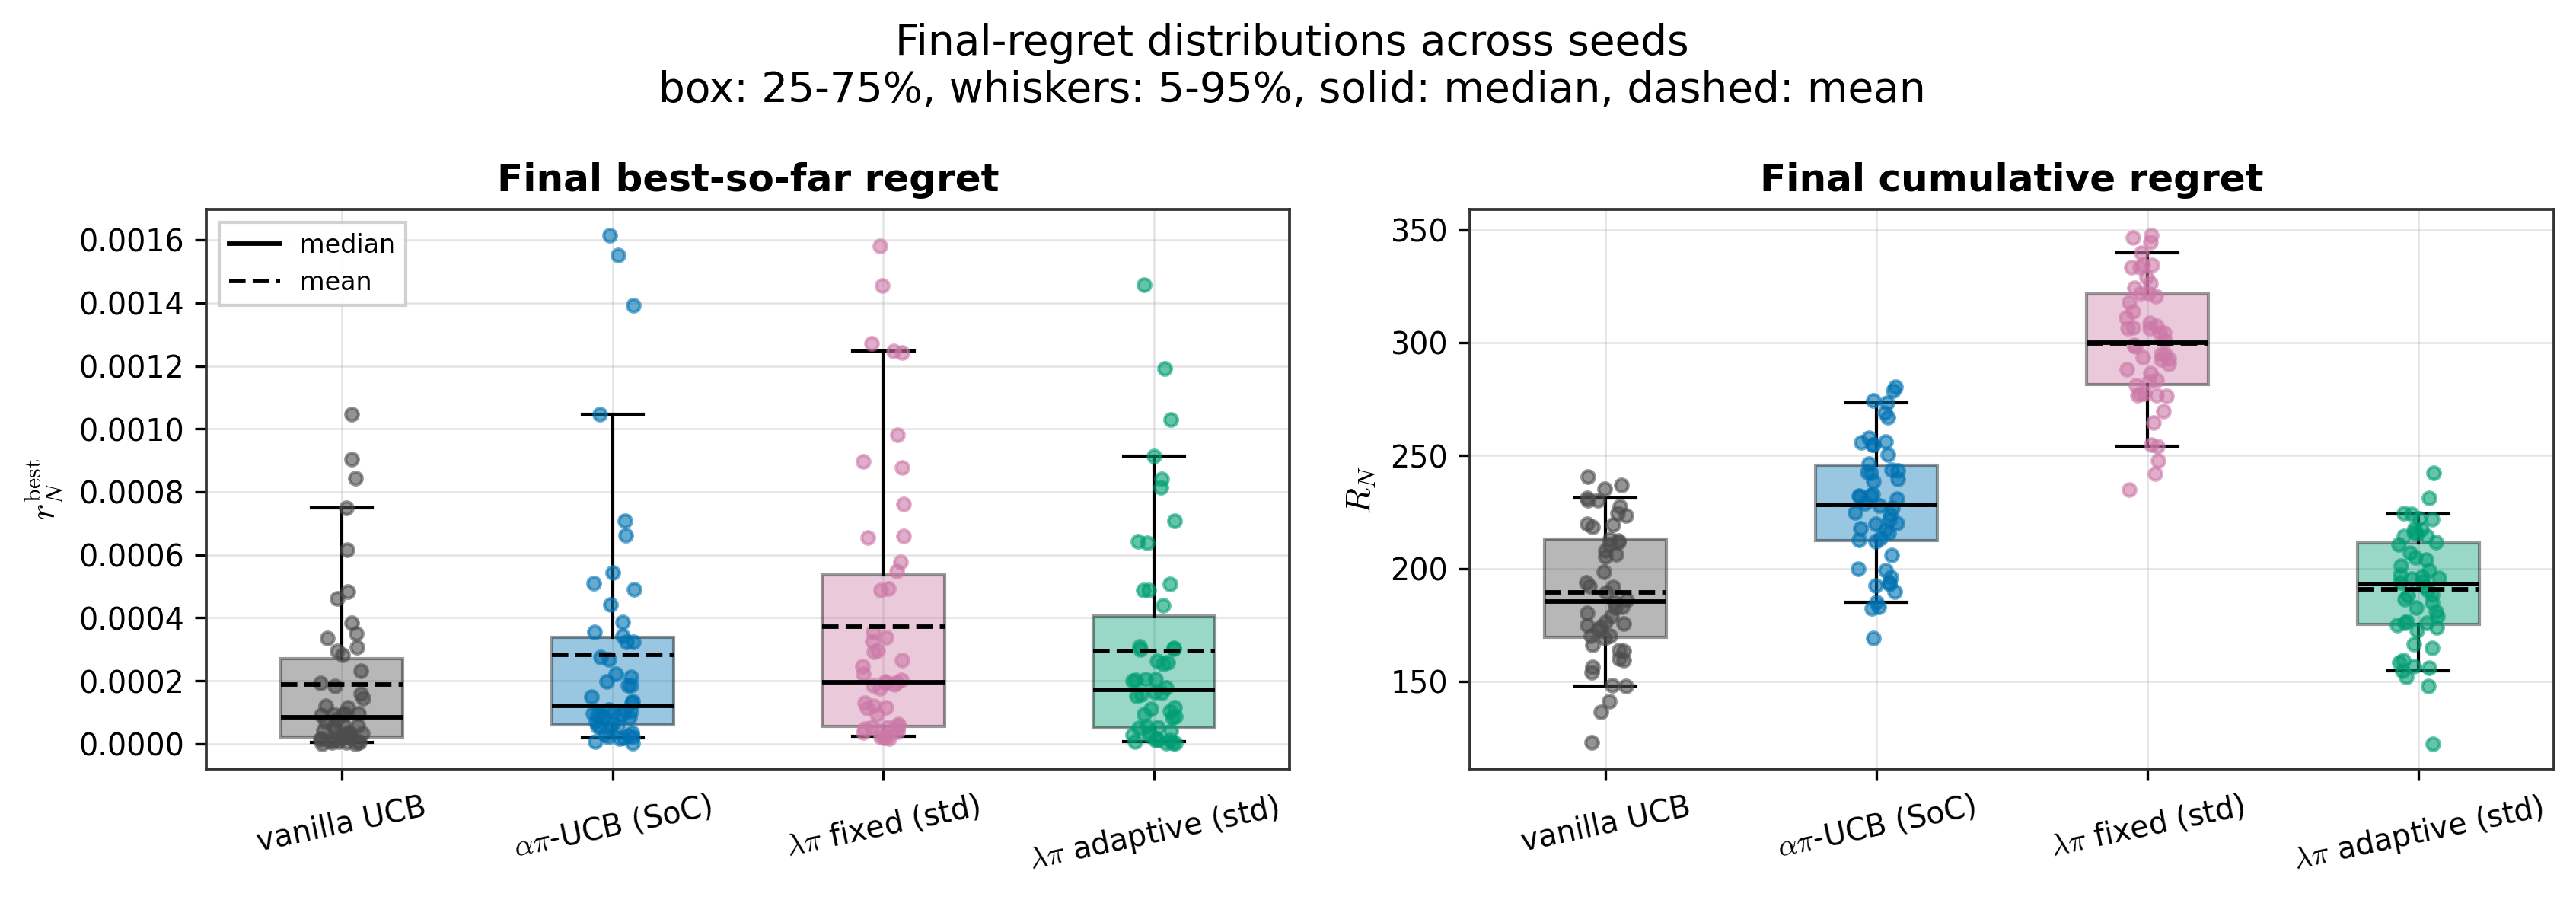
\includegraphics[
      width=\linewidth,
      keepaspectratio]{figures/EXPB/03_final_regret_distributions_branin_bad_prior.png}
    \caption{Final regret distribution, Branin 2-D.}
  \end{subfigure}
  \hfill
  \begin{subfigure}[b]{0.48\linewidth}
    \centering
    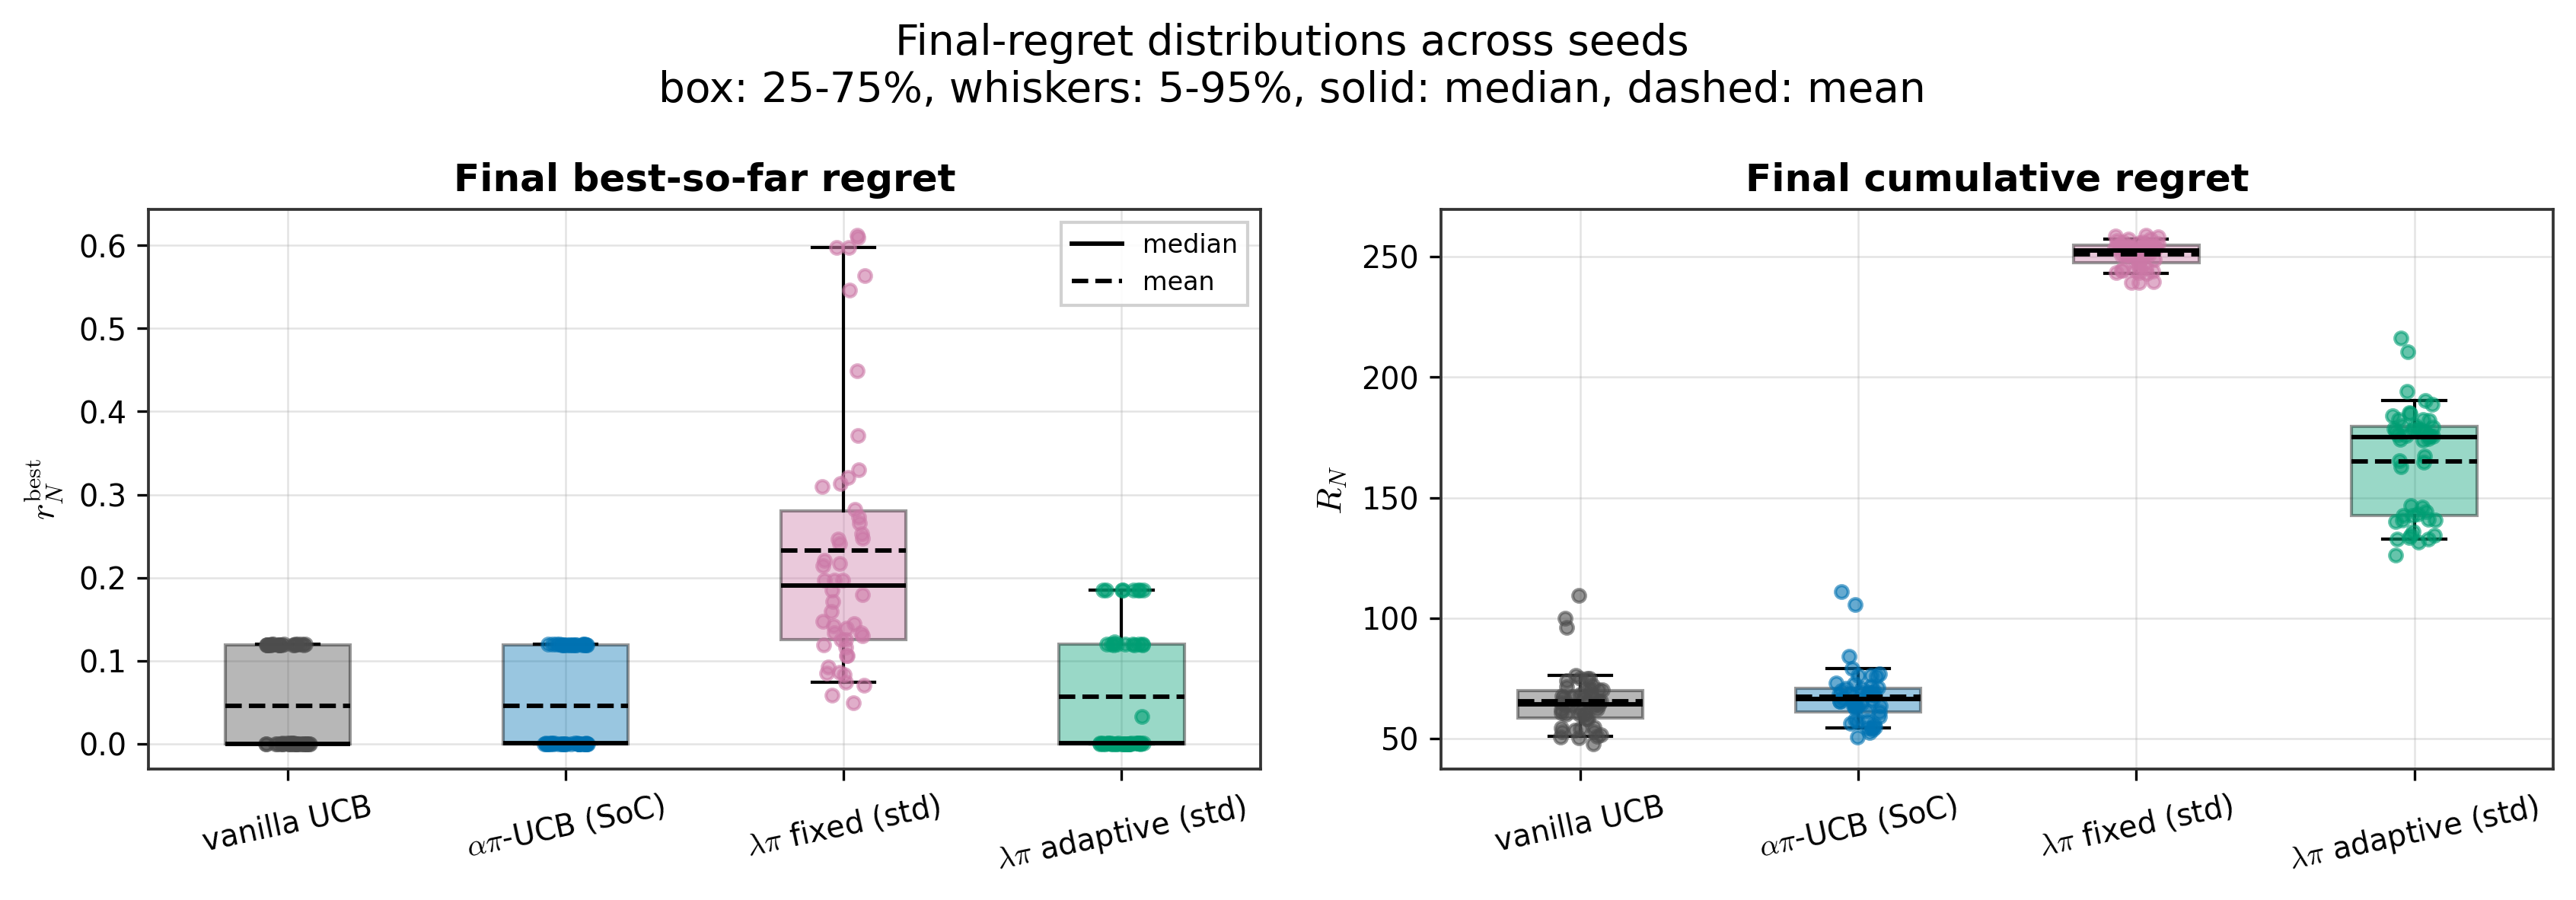
\includegraphics[
      width=\linewidth,
      keepaspectratio]{figures/EXPB/03_final_regret_distributions_hartmann_bad_prior.png}
    \caption{Final regret distribution, Hartmann 6-D.}
  \end{subfigure}

  \caption{\textbf{Final regret distributions across higher-dimensional benchmarks,
  Experiment~B.} Comparison of the acquisition-level and model-level uses of the
  functional prior on Branin (2-D) and Hartmann (6-D). Colours: grey $=$ vanilla,
  blue $=$ $\alpha$-$\pi$ (SoC), pink $=$ $\lambda$-$\pi$ fixed, green $=$
  $\lambda$-$\pi$ adaptive.}
  \label{fig:prior-final-regret}
\end{figure}

\begin{figure}[htbp]
  \centering

  \begin{subfigure}[b]{0.48\linewidth}
    \centering
    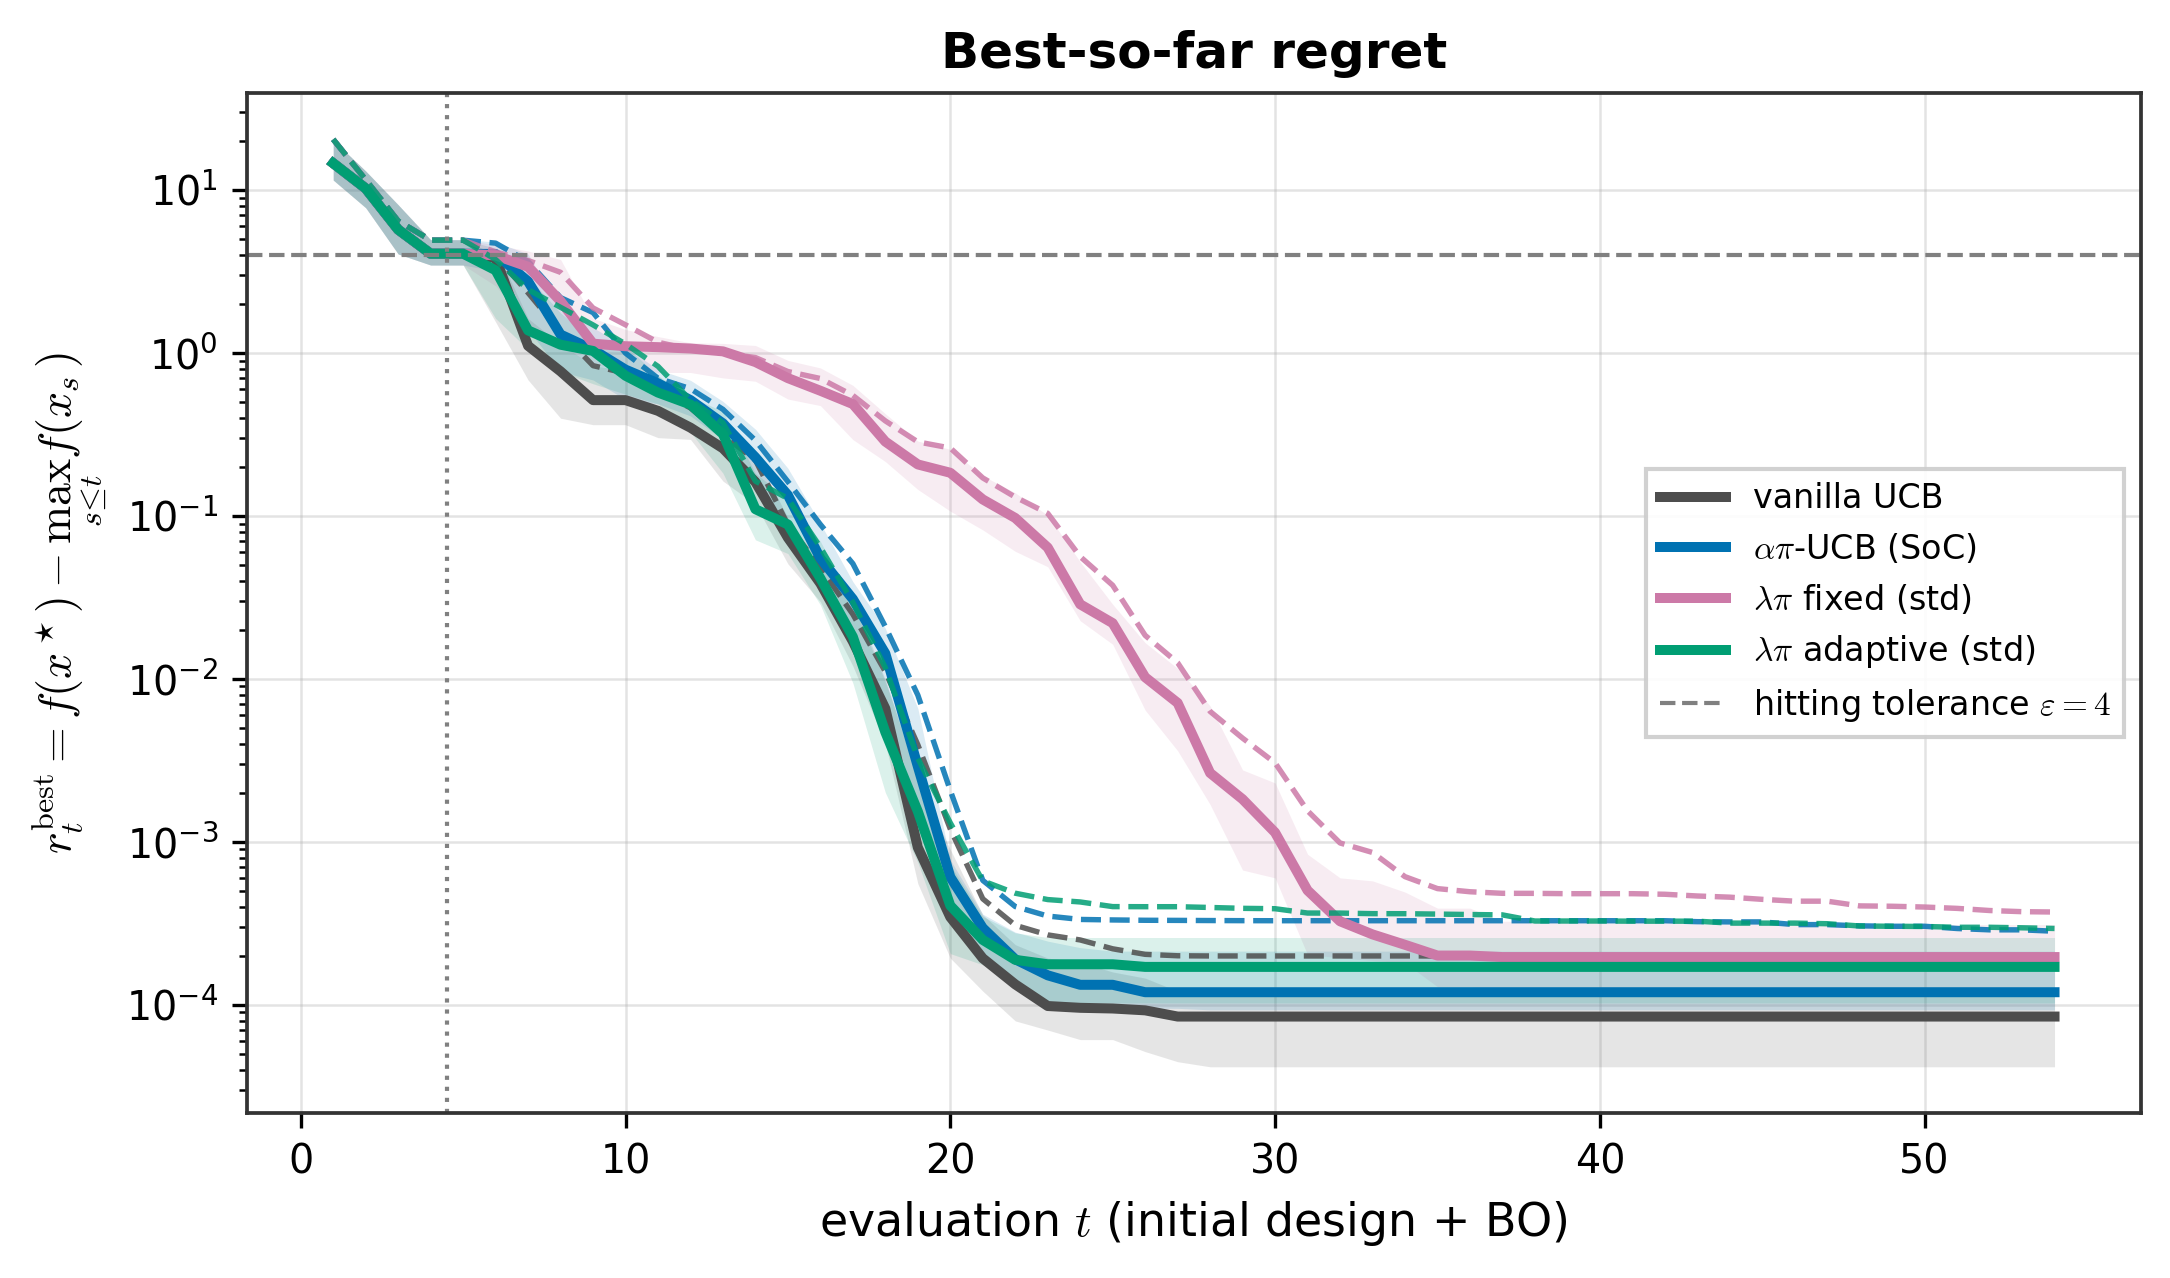
\includegraphics[
      width=\linewidth,
      keepaspectratio
    ]{figures/EXPB/03_best_so_far_regret_branin_bad_prior.png}
    \caption{Best-so-far regret, Branin 2-D.}
  \end{subfigure}
  \hfill
  \begin{subfigure}[b]{0.48\linewidth}
    \centering
    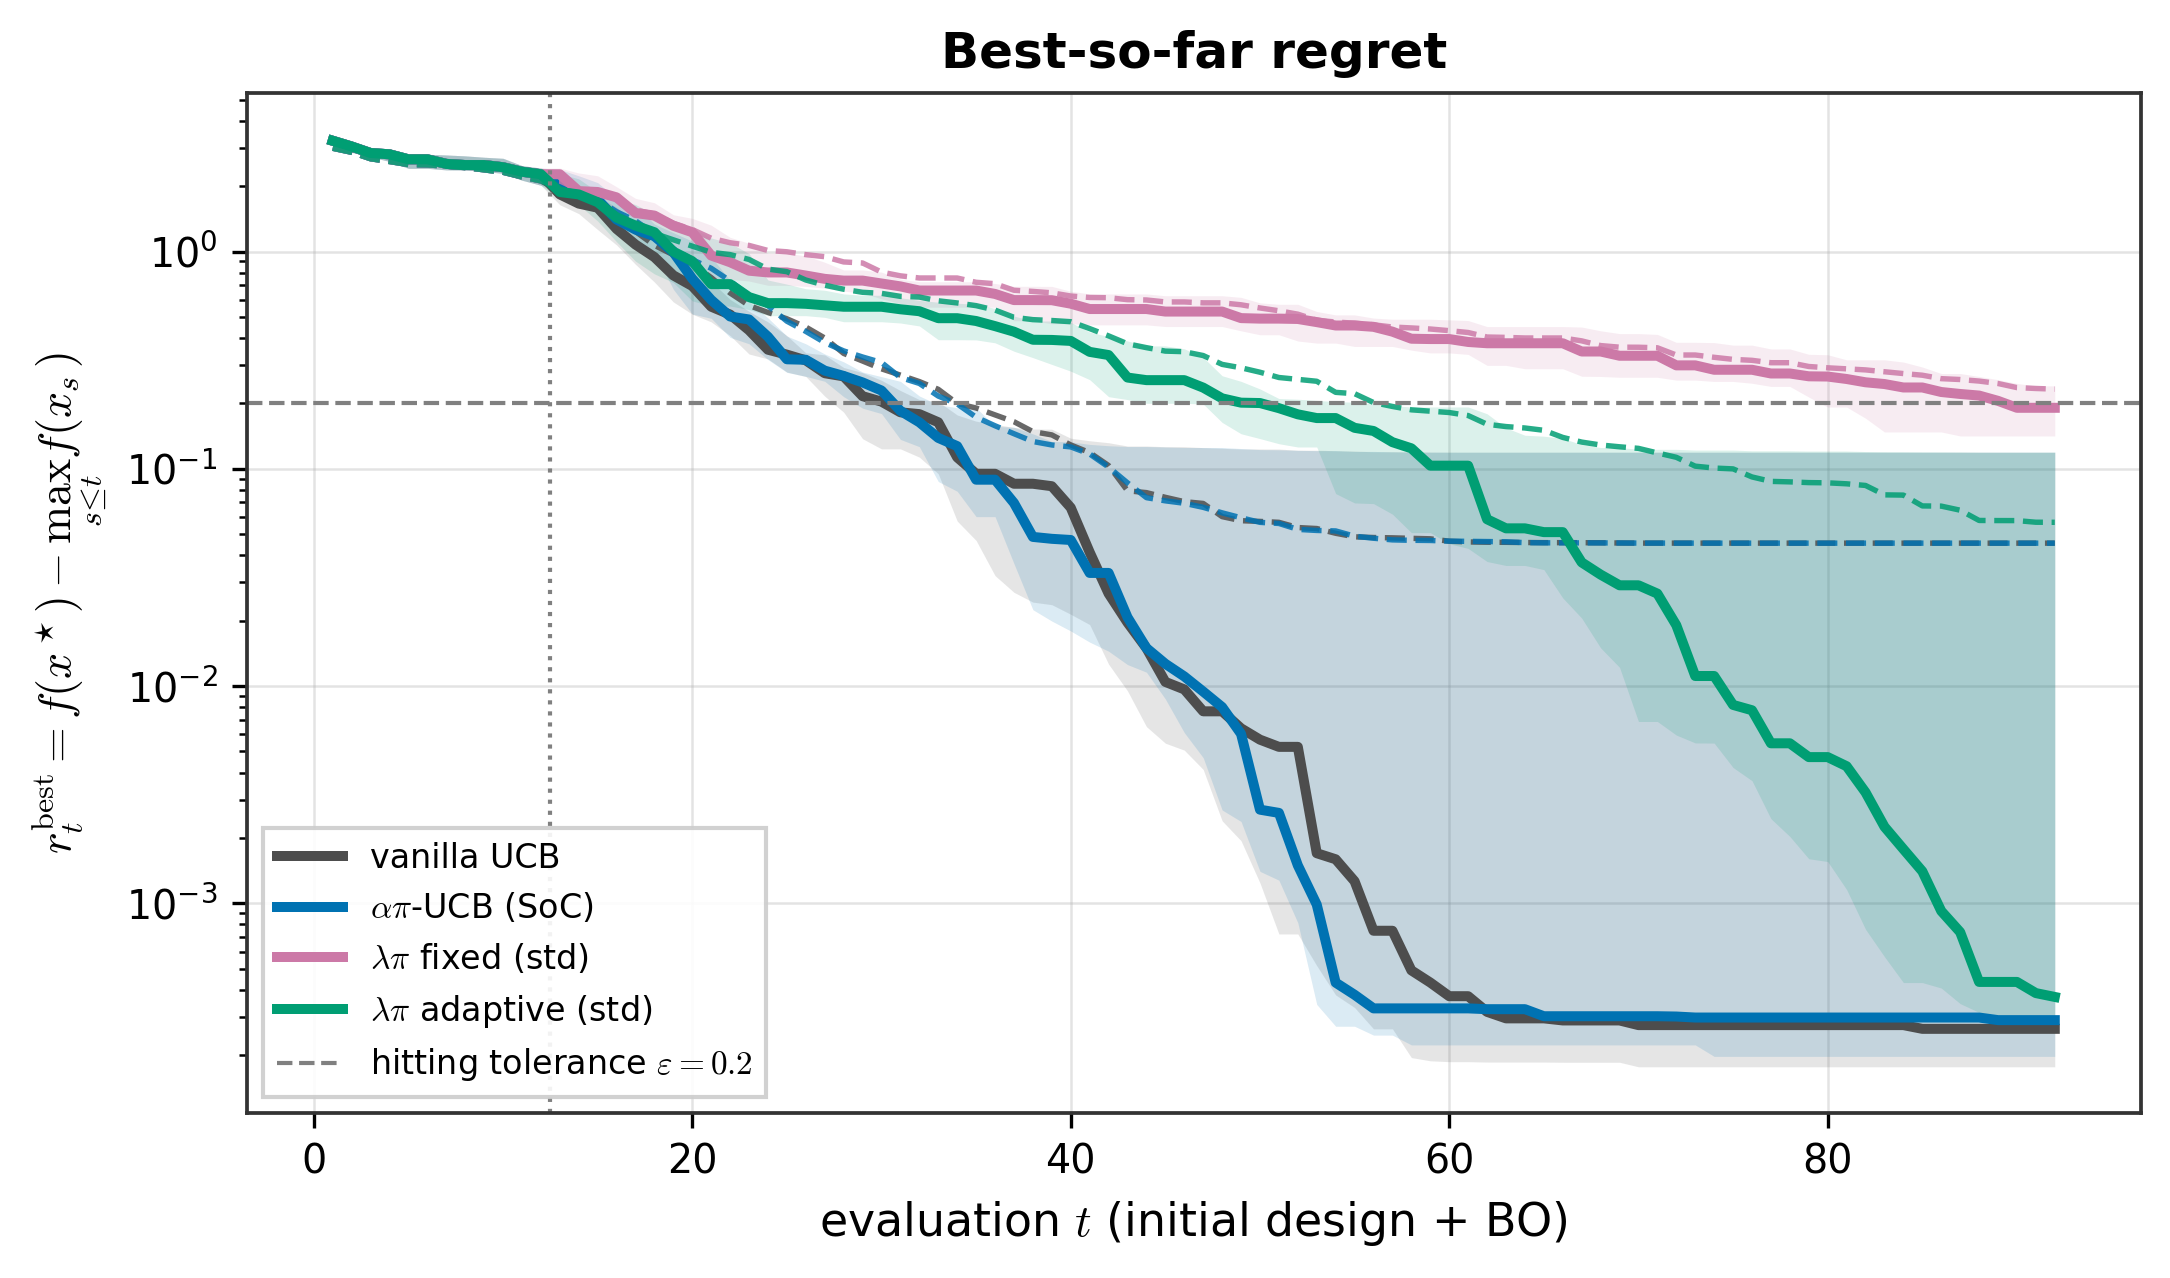
\includegraphics[
      width=\linewidth,
      keepaspectratio
    ]{figures/EXPB/03_best_so_far_regret_hartmann_bad_prior.png}
    \caption{Best-so-far regret, Hartmann 6-D.}
  \end{subfigure}

  \caption{\textbf{Best-so-far regret across higher-dimensional benchmarks,
  Experiment~B.} Comparison of the acquisition-level and model-level uses of the
  functional prior on Branin (2-D) and Hartmann (6-D). Colours: grey $=$ vanilla,
  blue $=$ $\alpha$-$\pi$ (SoC), pink $=$ $\lambda$-$\pi$ fixed, green $=$
  $\lambda$-$\pi$ adaptive.}
  \label{fig:prior-best-so-far-regret}
\end{figure}